\documentclass[12pt]{article}

\usepackage{sbc-template}
\usepackage[utf8]{inputenc}
\usepackage[T1]{fontenc}
\usepackage[brazil]{babel}
\usepackage{graphicx}
\usepackage{url}
\usepackage{booktabs}
\usepackage{array}
\usepackage{amsmath}
\usepackage{tikz}
\usetikzlibrary{positioning,arrows.meta,fit,backgrounds,calc}
\usepackage{pgfplots}
\pgfplotsset{compat=1.18}

\graphicspath{{figures/}}
\sloppy

% espaçamento um pouco mais justo em figuras e tabelas
\setlength{\textfloatsep}{10pt plus 2pt minus 2pt}
\setlength{\floatsep}{8pt plus 2pt minus 2pt}
\setlength{\intextsep}{8pt plus 2pt minus 2pt}

\tikzset{
  caixa/.style={draw, rounded corners=2pt, align=center, font=\scriptsize\sffamily,
                minimum height=8mm, inner sep=3pt, fill=#1},
  caixa/.default=white,
  seta/.style={-{Latex[length=2mm]}, thick},
  grupo/.style={draw, dashed, rounded corners=3pt, inner sep=4pt},
  rotulo/.style={font=\scriptsize\sffamily\bfseries}
}
\definecolor{azul}{HTML}{DCE6F2}
\definecolor{laranja}{HTML}{FBE3D0}
\definecolor{cinza}{HTML}{EEEEEE}
\definecolor{verde}{HTML}{DFF0D8}

\title{Manutenção preditiva com modelos clássicos e LLM:\\ um estudo comparativo na base AI4I 2020}

\author{Vitor Reis}

\address{Departamento de Ciência da Computação (DCC)\\
  Universidade Federal de Juiz de Fora (UFJF)\\
  Juiz de Fora -- MG -- Brasil
  % \email{seu.email@estudante.ufjf.br}
}

\begin{document}

\maketitle

\begin{resumo}
Este relatório compara modelos clássicos de aprendizado de máquina com um modelo de linguagem de grande porte (LLM) usado via \textit{prompting} na previsão de falhas de máquinas da base AI4I 2020, que reúne 10.000 ciclos de uma fresadora dos quais apenas 3,4\% terminam em falha. Na primeira etapa, SVM, MLP, Random Forest e XGBoost foram treinados em um \textit{pipeline} sem vazamento de informação, com padronização e SMOTE, e ajustados por busca em grade com validação cruzada de 5 \textit{folds}. Na segunda etapa, por sua vez, o modelo \texttt{deepseek-chat} classificou a mesma amostra fixa de 200 casos de teste sem exemplos (\textit{zero-shot}) e com 3, 5, 10 e 20 exemplos. Nessa amostra, enquanto os clássicos atingiram F1 entre 0,82 e 0,88, o LLM passou de 0,49 para 0,66, com revocação alta, mas com muitos alarmes falsos, cerca de 96~s por 100 amostras e custo estimado de US\$~0,12 para as 1.000 consultas. Conclui-se, portanto, que, havendo dados rotulados, os modelos clássicos vencem com folga, ao passo que o LLM serve sobretudo como triagem inicial quando ainda não há dados de treino.
\end{resumo}

% ---------------------------------------------------------------------------
\section{Introdução}

Em uma linha de produção, a parada não planejada de uma máquina interrompe a fabricação, atrasa entregas e, muitas vezes, danifica peças e ferramentas. Por esse motivo, a manutenção preditiva procura antecipar a falha a partir das leituras de sensores, de modo que a intervenção aconteça antes da quebra. Do ponto de vista de aprendizado de máquina, trata-se de uma classificação binária fortemente desbalanceada, já que a imensa maioria dos ciclos termina sem falha e, ainda assim, deixar passar uma falha custa muito mais do que emitir um alarme falso.

Tradicionalmente, esse problema é resolvido com modelos supervisionados, como SVM, redes MLP e conjuntos de árvores, treinados sobre milhares de exemplos rotulados. Mais recentemente, entretanto, os LLMs passaram a ser usados como classificadores genéricos, bastando descrever a tarefa em linguagem natural e, se for o caso, mostrar alguns exemplos no próprio \textit{prompt} \cite{brown2020,hegselmann2023}. Embora essa possibilidade seja atraente por dispensar treino, não é óbvio que ela funcione em dados tabulares, nos quais a decisão depende de limiares físicos. Diante disso, o objetivo deste trabalho é medir o ganho ou a perda de usar um LLM via \textit{prompting} em vez de modelos clássicos, na mesma tarefa e sobre os mesmos dados. A Figura~\ref{fig:pipeline} resume o experimento como um todo.

\begin{figure}[ht]
\centering
\begin{tikzpicture}[node distance=4mm and 5mm]
  \node[caixa=cinza] (csv) {AI4I 2020\\10.000 ciclos};
  \node[caixa=cinza, right=of csv] (limpa) {limpeza\\$-$UDI, ID\\$-$modos de falha};
  \node[caixa=cinza, right=of limpa] (split) {divisão 80/20\\estratificada\\semente 42};
  \node[caixa=cinza, above right=1mm and 6mm of split] (treino) {treino\\8.000 (271 falhas)};
  \node[caixa=cinza, below right=1mm and 6mm of split] (teste) {teste\\2.000 (68 falhas)};
  \node[caixa=verde, right=6mm of teste] (amostra) {amostra fixa\\200 (50 falhas)};
  % Etapa I
  \node[caixa=azul, above=9mm of treino, xshift=-26mm] (prep) {one-hot + \\ z-score};
  \node[caixa=azul, right=of prep] (smote) {SMOTE};
  \node[caixa=azul, right=of smote] (clf) {SVM / MLP\\RF / XGB};
  \node[caixa=azul, right=of clf] (gs) {GridSearch\\5 \textit{folds}, F1};
  \begin{scope}[on background layer]
    \node[grupo, fit=(prep)(smote)(clf)(gs), label={[rotulo]above:Etapa I: \textit{pipeline} ajustado só no treino}] (e1) {};
  \end{scope}
  % Etapa II
  \node[caixa=laranja, below=9mm of teste, xshift=-30mm] (fs) {$k\in\{0,3,5,10,20\}$\\exemplos do treino};
  \node[caixa=laranja, right=of fs] (pr) {\textit{prompt} v1\\(texto)};
  \node[caixa=laranja, right=of pr] (api) {DeepSeek API\\temperatura 0};
  \node[caixa=laranja, right=of api] (js) {JSON\\falha, prob.};
  \begin{scope}[on background layer]
    \node[grupo, fit=(fs)(pr)(api)(js), label={[rotulo]below:Etapa II: classificação via \textit{prompting}}] (e2) {};
  \end{scope}
  \node[caixa=verde, right=8mm of amostra] (met) {métricas\\acurácia, P, R\\F1, AUC, MC\\tempo, custo};
  \draw[seta] (csv) -- (limpa); \draw[seta] (limpa) -- (split);
  \draw[seta] (split) |- (treino); \draw[seta] (split) |- (teste);
  \draw[seta] (teste) -- (amostra);
  \draw[seta] (treino.north) -- (treino.north |- e1.south);
  \draw[seta] (prep) -- (smote); \draw[seta] (smote) -- (clf); \draw[seta] (clf) -- (gs);
  \draw[seta] (fs) -- (pr); \draw[seta] (pr) -- (api); \draw[seta] (api) -- (js);
  \draw[seta] (treino.east) -- ++(3mm,0) |- ($(teste.south)!0.5!(fs.north)$) -| (fs.north);
  \draw[seta] (amostra.south) -- (amostra.south |- api.north) node[pos=0.5, right, font=\tiny\sffamily] {consultas};
  \draw[seta] (gs.east) -| (met.north);
  \draw[seta] (js.east) -| (met.south);
  \draw[seta] (amostra) -- (met);
\end{tikzpicture}
\caption{Visão geral do experimento. Os dois estágios são avaliados na mesma amostra fixa; os clássicos também são avaliados no teste completo.}
\label{fig:pipeline}
\end{figure}

% ---------------------------------------------------------------------------
\section{Problema e base de dados}\label{sec:base}

A base escolhida foi a AI4I 2020 \textit{Predictive Maintenance Dataset} \cite{matzka2020,matzka2020uci}, que, embora sintética, foi construída para reproduzir o comportamento de uma fresadora real. Cada um dos seus 10.000 ciclos é descrito por seis atributos de entrada: o tipo do produto (L, M ou H, presentes em cerca de 60\%, 30\% e 10\% dos ciclos), as temperaturas do ar e do processo [K], a rotação [rpm], o torque [N$\cdot$m] e o desgaste da ferramenta [min]. O valor desejado, \textit{Machine failure}, vale 1 em apenas 339 ciclos (3,39\%); consequentemente, um classificador que sempre respondesse ``normal'' acertaria 96,6\% dos casos sem detectar falha alguma, o que mostra que a acurácia, sozinha, não serve como métrica aqui. A Tabela~\ref{tab:exemplos} traz três exemplos reais: enquanto os dois primeiros são ciclos normais, o terceiro é uma falha de potência, causada por uma rotação muito alta combinada com um torque muito baixo.

\begin{table}[ht]
\centering
\caption{Exemplos da base AI4I 2020 (UDI 1, 2 e 51).}
\label{tab:exemplos}
\small\setlength{\tabcolsep}{3.5pt}
\begin{tabular}{cccccccc}
\toprule
UDI & Tipo & T. ar [K] & T. processo [K] & Rotação [rpm] & Torque [N$\cdot$m] & Desgaste [min] & Falha \\
\midrule
1  & M & 298,1 & 308,6 & 1551 & 42,8 & 0   & 0 \\
2  & L & 298,2 & 308,7 & 1408 & 46,3 & 3   & 0 \\
51 & L & 298,9 & 309,1 & 2861 & 4,6  & 143 & 1 \\
\bottomrule
\end{tabular}
\end{table}

Como se vê na Figura~\ref{fig:eda}, as falhas se concentram em torques muito altos ou muito baixos, em rotações extremas e em desgastes elevados; contudo, nenhuma variável isolada separa as classes, o que justifica o uso de modelos que combinem os atributos. Além disso, a base traz cinco colunas que indicam o modo da falha (TWF, HDF, PWF, OSF e RNF). Como essas colunas só valem 1 quando a falha já ocorreu, usá-las como entrada entregaria a resposta ao modelo; por isso, elas foram retiradas da entrada e mantidas apenas para a análise dos erros.

\begin{figure}[ht]
\centering
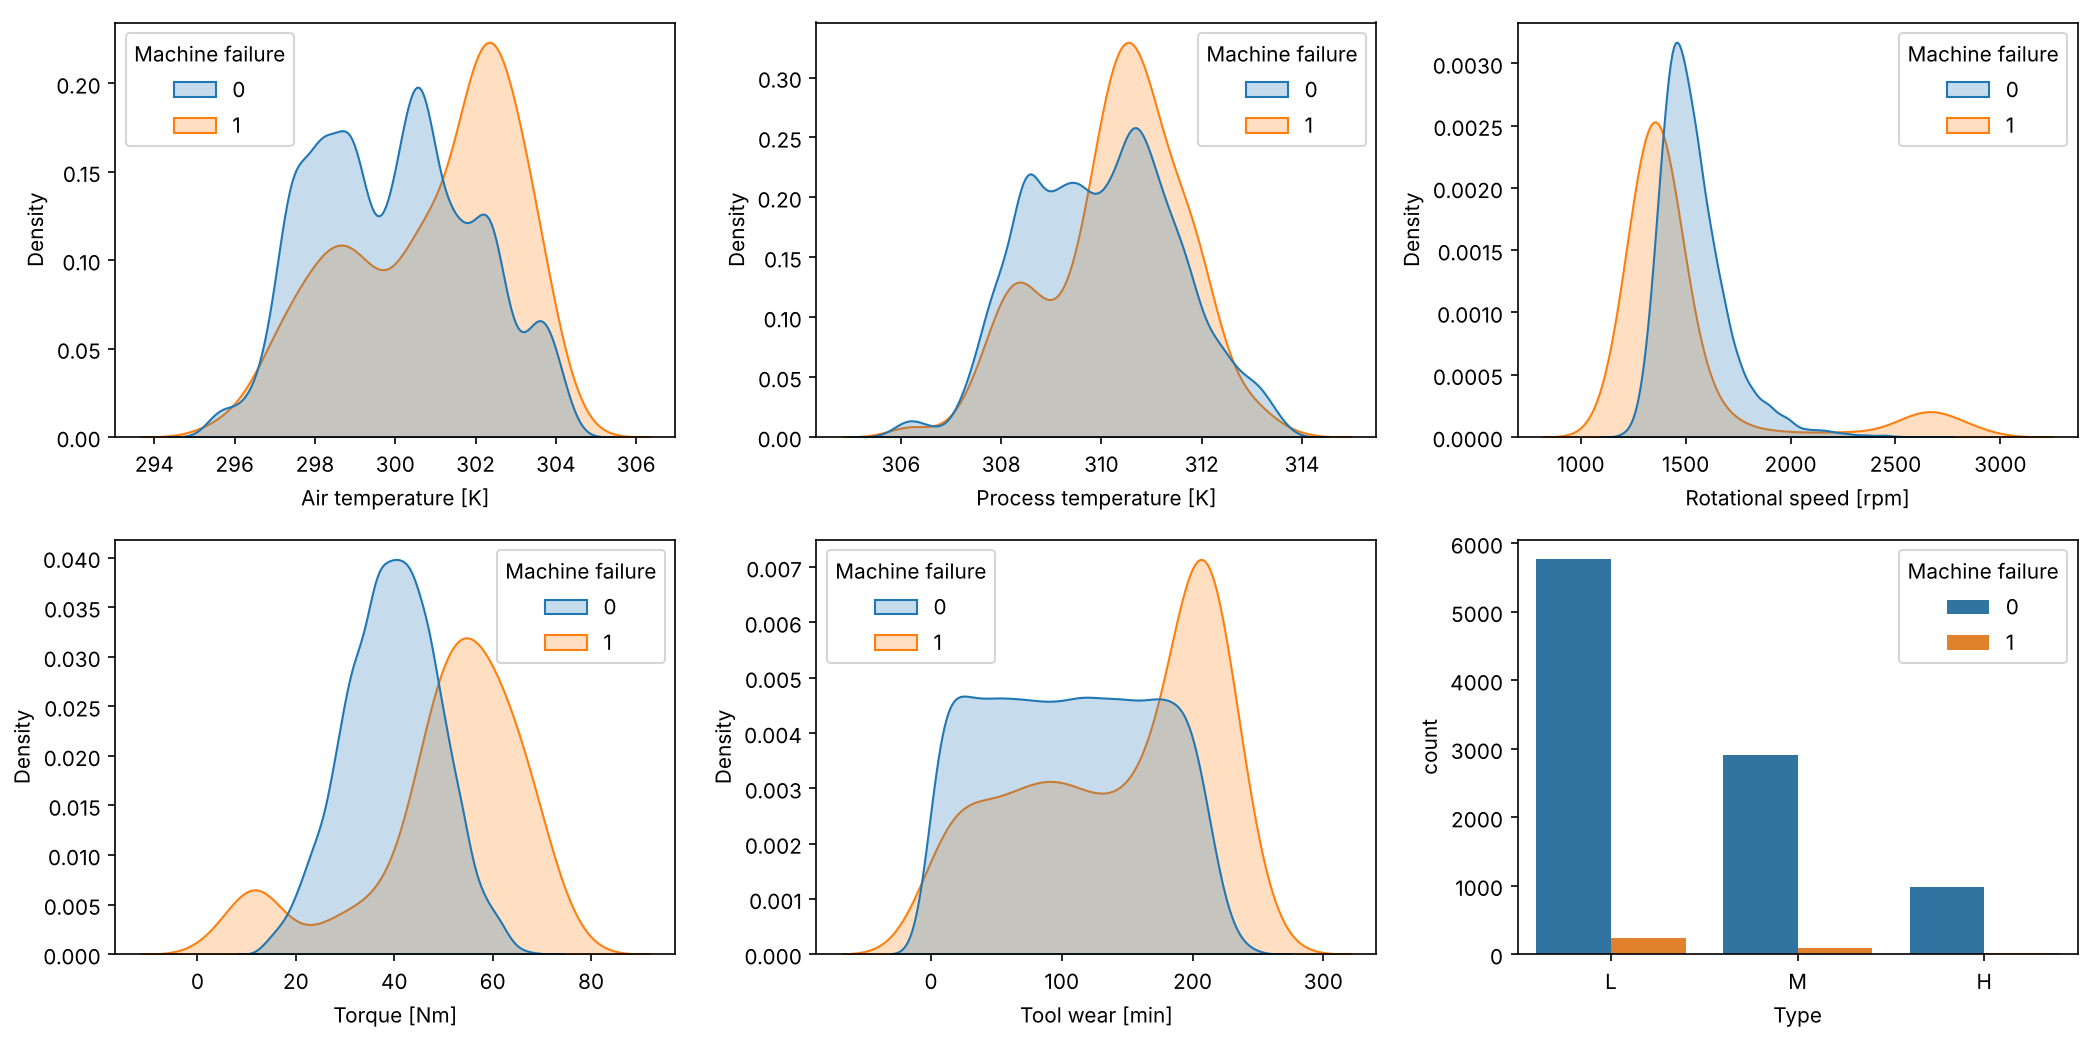
\includegraphics[width=\textwidth]{eda_distribuicoes.png}
\caption{Distribuição dos atributos numéricos por classe (gerada em \texttt{01\_eda\_preparacao.ipynb}).}
\label{fig:eda}
\end{figure}

% ---------------------------------------------------------------------------
\section{Metodologia}\label{sec:metodo}

Inicialmente, verificou-se que a base não tem valores nulos nem registros duplicados. Em seguida, foram descartados os identificadores \textit{UDI} e \textit{Product ID}, que não carregam informação física, além dos modos de falha. O atributo \textit{Type} foi então codificado por \textit{one-hot}, ao passo que os atributos numéricos foram padronizados por \textit{z-score}. Vale destacar que essa padronização foi feita dentro do \textit{pipeline} de cada modelo, de modo que a média e o desvio padrão são estimados apenas com os dados de treino de cada \textit{fold}.

Para lidar com o desbalanceamento, utilizou-se o SMOTE \cite{chawla2002}, que cria falhas sintéticas por interpolação entre vizinhos próximos. Da mesma forma que a padronização, ele foi colocado no \textit{pipeline} do \textit{imbalanced-learn} \cite{lemaitre2017}; assim, as falhas sintéticas surgem apenas nos \textit{folds} de treino e nunca contaminam a validação ou o teste.

Quanto à divisão dos dados, adotou-se uma separação 80/20 estratificada com semente 42, o que resultou em 8.000 ciclos de treino (271 falhas) e 2.000 de teste (68 falhas); os hiperparâmetros, por sua vez, foram escolhidos apenas por validação cruzada no treino. Como cada consulta ao LLM leva cerca de 1~s e tem custo, e como uma subamostra estratificada de 200 casos teria apenas 7 falhas, sorteou-se do teste uma \textbf{amostra fixa enriquecida} de 200 casos, com 50 falhas e 150 ciclos normais, avaliada por todos os modelos. Entretanto, como esse enriquecimento infla a precisão, os modelos clássicos também foram avaliados no teste completo.

Por fim, seguindo o enunciado, foram calculadas acurácia, precisão, revocação, F1, AUC-ROC e matriz de confusão, sempre com a falha como classe positiva. Nesse contexto, a revocação indica quantas falhas reais foram detectadas, enquanto a precisão indica quantos alarmes eram de fato falhas. Por equilibrar as duas, o F1 da classe falha foi adotado como métrica principal, tanto na busca em grade quanto na comparação. Na Etapa~II, além disso, foram medidos o tempo por 100 amostras, os tokens consumidos e o custo da API.

% ---------------------------------------------------------------------------
\section{Etapa I: algoritmos clássicos}\label{sec:etapa1}

Dentre os modelos sugeridos, foram escolhidos a SVM com \textit{kernel} RBF \cite{cortes1995} e a MLP \cite{haykin2009}, que correspondem ao conteúdo central da disciplina, e, como referência, o Random Forest \cite{breiman2001} e o XGBoost \cite{chen2016}, que costumam ser fortes em dados tabulares. Todos foram implementados com \textit{scikit-learn} \cite{pedregosa2011} e ajustados por \textit{GridSearchCV} com validação cruzada estratificada de 5 \textit{folds}, otimizando o F1; a MLP, em particular, foi treinada com até 500 épocas e parada antecipada. A Tabela~\ref{tab:grade} resume a grade testada, a melhor configuração de cada modelo e o tempo da busca.

\begin{table}[ht]
\centering
\caption{Grade de hiperparâmetros, melhor configuração, F1 médio na validação cruzada e tempo da busca.}
\label{tab:grade}
\footnotesize
\begin{tabular}{l>{\raggedright}p{4.9cm}>{\raggedright}p{3.6cm}cc}
\toprule
Modelo & Grade testada & Melhor configuração & F1 (CV) & Busca [s] \tabularnewline
\midrule
SVM (RBF) & $C \in \{0{,}1;1;10;100\}$, $\gamma \in \{\text{scale};0{,}1;0{,}01\}$ & $C=100$, $\gamma=$ scale & 0,542 & 186,8 \tabularnewline
MLP & camadas $\in \{(16),(32),(32,16),(64,32)\}$, $\alpha \in \{10^{-4},10^{-3},10^{-2}\}$, taxa $\in \{10^{-3},10^{-2}\}$ & $(64,32)$, $\alpha=10^{-2}$, taxa $10^{-2}$ & 0,594 & 81,2 \tabularnewline
Random Forest & árvores $\in \{200,500\}$, profundidade $\in \{\text{livre},10,20\}$ & 200, livre & 0,631 & 18,5 \tabularnewline
XGBoost & árvores $\in \{200,500\}$, prof. $\in \{3,6\}$, taxa $\in \{0{,}05;0{,}1\}$ & 500, prof. 6, taxa 0,1 & 0,689 & 8,4 \tabularnewline
\bottomrule
\end{tabular}
\end{table}

No teste completo (Tabela~\ref{tab:teste}), todos os modelos detectam entre 74\% e 81\% das falhas e alcançam AUC-ROC entre 0,95 e 0,97 (Figura~\ref{fig:roc}), o que mostra que separam bem as classes. No entanto, eles diferem bastante na quantidade de alarmes falsos: enquanto o XGBoost emite apenas 22 e obtém o melhor F1 (0,76), a SVM emite 79 e fica com 0,53 (Figura~\ref{fig:cmclass}). Esse resultado é coerente com a natureza da base, cujas falhas seguem regras de limiar, um tipo de fronteira que os conjuntos de árvores aproximam com facilidade.

\begin{table}[ht]
\centering
\caption{Etapa I no teste completo (2.000 ciclos, 68 falhas).}
\label{tab:teste}
\small\setlength{\tabcolsep}{3.5pt}
\begin{tabular}{lccccccccc}
\toprule
Modelo & Acurácia & Precisão & Revocação & F1 & AUC-ROC & VN & FP & FN & VP \\
\midrule
SVM           & 0,953 & 0,402 & 0,779 & 0,530 & 0,951 & 1853 & 79 & 15 & 53 \\
MLP           & 0,967 & 0,509 & 0,809 & 0,625 & 0,969 & 1879 & 53 & 13 & 55 \\
Random Forest & 0,966 & 0,495 & 0,735 & 0,592 & 0,973 & 1881 & 51 & 18 & 50 \\
XGBoost       & \textbf{0,983} & \textbf{0,714} & \textbf{0,809} & \textbf{0,759} & 0,970 & 1910 & 22 & 13 & 55 \\
\bottomrule
\end{tabular}
\end{table}

\begin{figure}[ht]
\centering
\begin{minipage}[b]{.47\textwidth}\centering
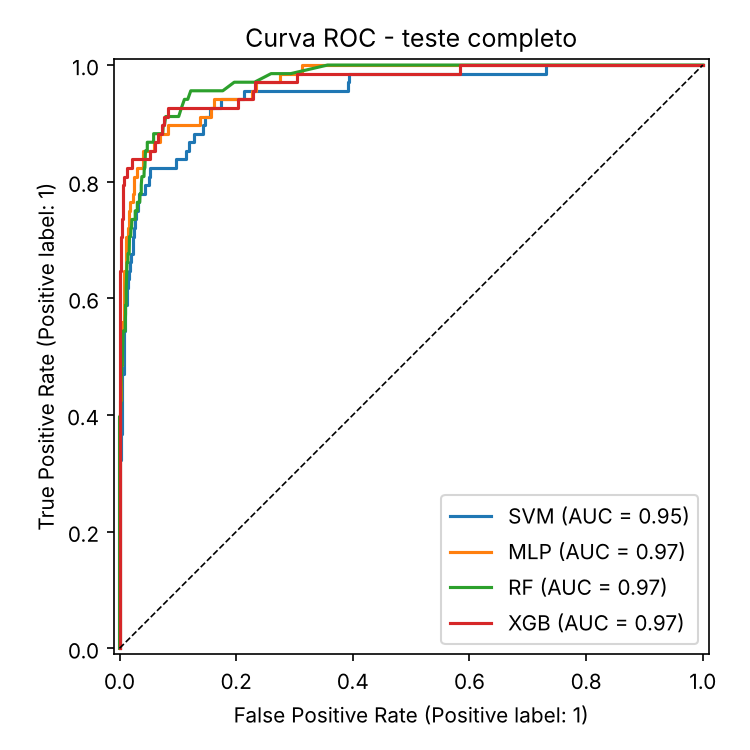
\includegraphics[width=\linewidth]{roc_classical.png}
\caption{Curvas ROC no teste completo.}
\label{fig:roc}
\end{minipage}\hfill
\begin{minipage}[b]{.5\textwidth}\centering
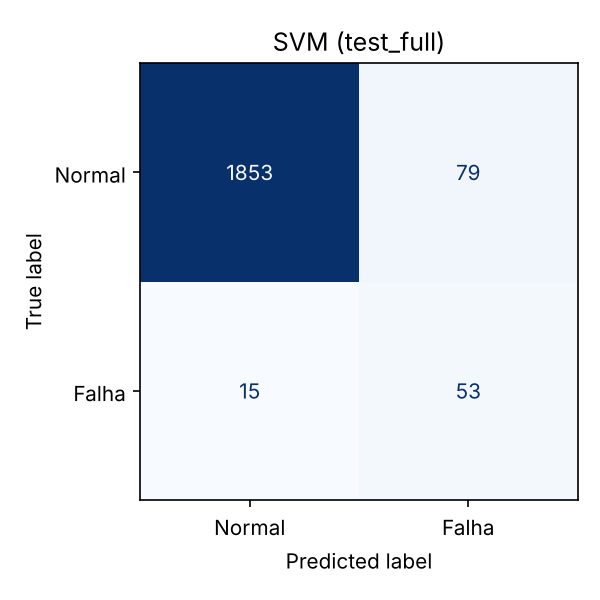
\includegraphics[width=.49\linewidth]{cm_svm_test_full.png}\hfill
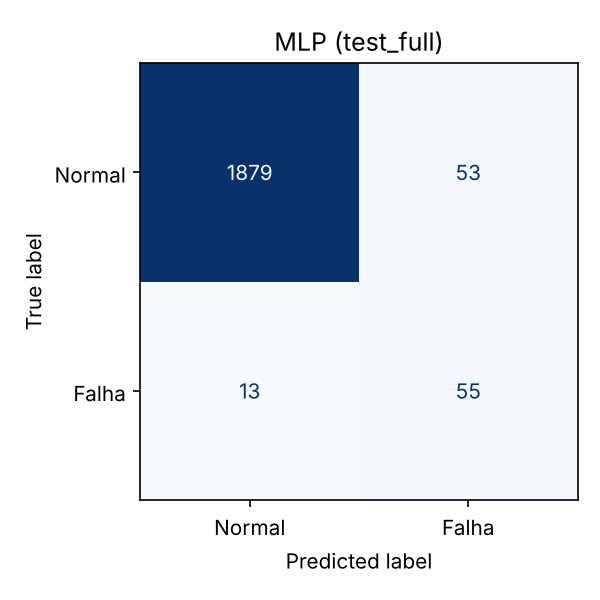
\includegraphics[width=.49\linewidth]{cm_mlp_test_full.png}\\[1mm]
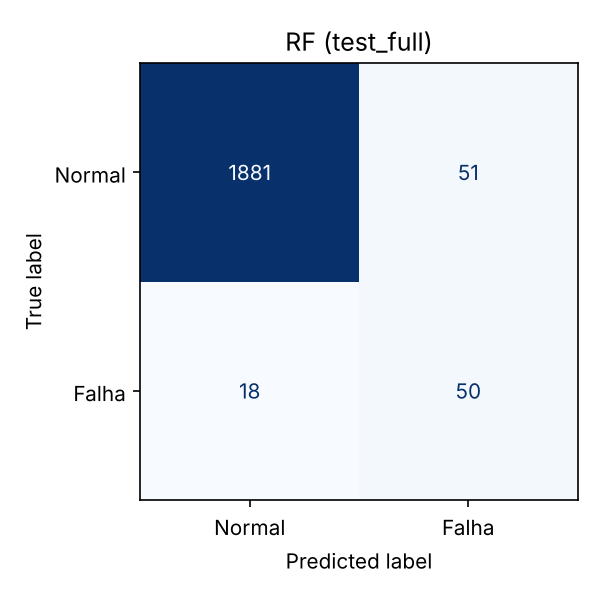
\includegraphics[width=.49\linewidth]{cm_rf_test_full.png}\hfill
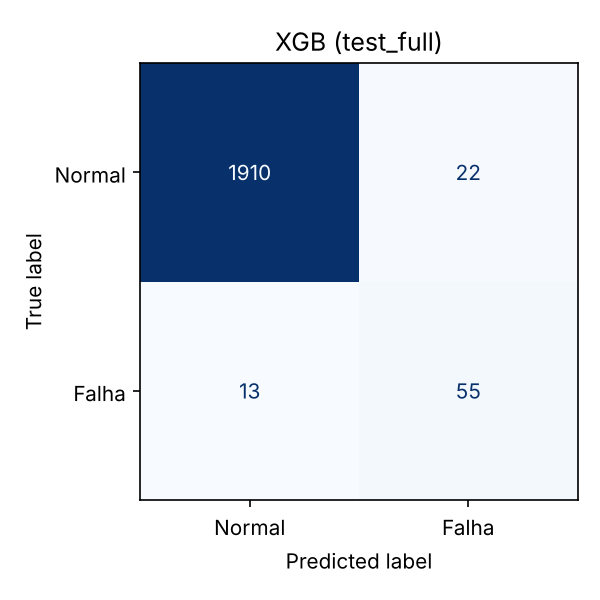
\includegraphics[width=.49\linewidth]{cm_xgb_test_full.png}
\caption{Matrizes de confusão no teste completo: SVM, MLP, RF e XGBoost.}
\label{fig:cmclass}
\end{minipage}
\end{figure}

Já na amostra fixa (Tabela~\ref{tab:comparacao}), os números sobem: MLP e XGBoost chegam a F1 0,88, a SVM a 0,87 e o RF a 0,82. Essa melhora, porém, não reflete modelos melhores, e sim o enriquecimento da amostra, pois, com 25\% de falhas, há bem menos ciclos normais que possam virar alarme falso. Por isso, esses valores servem para comparar modelos entre si, mas não como desempenho esperado em operação.

Além da configuração principal, foram testadas duas variações (Figura~\ref{fig:variacoes}). Na primeira, o SMOTE foi trocado por pesos de classe; na segunda, mantido o SMOTE, acrescentaram-se três atributos derivados das regras da base, a saber, a diferença de temperatura, a potência (torque $\times$ velocidade angular) e o produto desgaste $\times$ torque. Os atributos derivados ajudam SVM, MLP e, sobretudo, o RF, cujo F1 sobe de 0,59 para 0,72, o que confirma que as falhas dependem dessas grandezas. Os pesos de classe, por outro lado, favorecem as árvores, de modo que o XGBoost chega a 0,768; já a MLP, como o \texttt{MLPClassifier} não aceita pesos, acabou treinada sem balanceamento e ficou conservadora demais (revocação 0,46). Ainda assim, a comparação com o LLM usa a configuração principal, para que os dois estágios recebam as mesmas seis grandezas brutas.

\begin{figure}[ht]
\centering
\begin{tikzpicture}
\begin{axis}[
  ybar, bar width=7pt, width=.82\textwidth, height=4.6cm,
  symbolic x coords={SVM,MLP,Random Forest,XGBoost}, xtick=data,
  ymin=0.4, ymax=0.95, ytick={0.4,0.5,0.6,0.7,0.8,0.9}, ylabel={F1 (teste completo)},
  ticklabel style={font=\scriptsize}, label style={font=\scriptsize},
  legend style={font=\scriptsize, at={(0.5,-0.22)}, anchor=north, legend columns=3, draw=none},
  nodes near coords, nodes near coords style={font=\tiny, rotate=90, anchor=west},
  /pgf/number format/.cd, fixed, fixed zerofill, precision=2, use comma,
  enlarge x limits=0.15]
\addplot[fill=blue!35] coordinates {(SVM,0.530) (MLP,0.625) (Random Forest,0.592) (XGBoost,0.759)};
\addplot[fill=gray!40] coordinates {(SVM,0.493) (MLP,0.596) (Random Forest,0.692) (XGBoost,0.768)};
\addplot[fill=green!40!black!30] coordinates {(SVM,0.559) (MLP,0.640) (Random Forest,0.718) (XGBoost,0.748)};
\legend{SMOTE (principal), pesos de classe, SMOTE + derivados}
\end{axis}
\end{tikzpicture}
\caption{F1 no teste completo para cada estratégia de balanceamento e conjunto de atributos (\texttt{summary.csv}).}
\label{fig:variacoes}
\end{figure}

% ---------------------------------------------------------------------------
\section{Etapa II: LLM via \textit{prompting}}\label{sec:etapa2}

Na segunda etapa, utilizou-se o modelo \texttt{deepseek-chat} pela API da DeepSeek \cite{deepseek2026}, com temperatura zero e até 200 tokens de saída. As consultas foram feitas em sequência em 22/11/2026, e as métricas foram depois regeneradas a partir do cache das respostas, em 26/11/2026. Cabe ressaltar que \texttt{deepseek-chat} é um apelido: segundo o histórico da DeepSeek, desde abril de 2026 ele aponta para o \texttt{deepseek-v4-flash} sem raciocínio estendido, mas, como a API não registrou a versão exata, essa correspondência é uma inferência.

O \textit{prompt} (versão v1), escrito em português, segue a estrutura da Figura~\ref{fig:prompt}. Primeiro, a mensagem de sistema define o papel do modelo (engenheiro de manutenção de fresadoras), explica os atributos e exige como resposta um JSON com o rótulo e uma probabilidade, a qual permite calcular a AUC-ROC. Em seguida, a mensagem de usuário traz os exemplos, quando houver, e a leitura a classificar. Os exemplos vêm do treino, sendo metade falhas (no mínimo uma), e são aninhados ($3 \subset 5 \subset 10 \subset 20$), de forma que cada configuração apenas acrescenta exemplos à anterior.

\begin{figure}[ht]
\centering
\begin{tikzpicture}[node distance=3mm]
  \node[caixa=laranja, text width=4.3cm, align=left] (sys) {\textbf{Sistema}\\Papel: engenheiro de manutenção\\Tarefa: falha (1) ou não (0)\\Significado dos 6 atributos\\Saída: somente JSON};
  \node[caixa=cinza, text width=5.6cm, align=left, right=6mm of sys, yshift=5mm] (ex) {\textbf{Usuário: exemplos} ($k$ = 0, 3, 5, 10, 20)\\\texttt{- Tipo: L | Temperatura do ar: 302.4 K | ...\\\ \ Desgaste: 163 min -> \{"falha": 1\}}};
  \node[caixa=cinza, text width=5.6cm, align=left, below=of ex] (q) {\textbf{Usuário: consulta}\\\texttt{Classifique esta leitura: Tipo: M | ...}};
  \node[caixa=verde, right=6mm of q, text width=2.6cm] (out) {\texttt{\{"falha": 1,\\"probabilidade": 0.82\}}};
  \draw[seta] (sys.east) -- ++(3mm,0) |- (ex.west);
  \draw[seta] (ex) -- (q); \draw[seta] (q) -- (out);
\end{tikzpicture}
\caption{Estrutura do \textit{prompt}. No \textit{zero-shot} o bloco de exemplos é omitido; os \textit{prompts} completos ficam em \texttt{reports/results/prompts/}.}
\label{fig:prompt}
\end{figure}

Em todas as 1.000 consultas (200 casos $\times$ 5 configurações), o modelo devolveu um JSON válido. Como mostram a Tabela~\ref{tab:llm} e a Figura~\ref{fig:fk}, porém, o LLM é alarmista: no \textit{zero-shot}, ele detecta 86\% das falhas, mas marca 83 dos 150 ciclos normais como falha, o que resulta em F1 de 0,49. À medida que exemplos são acrescentados, os alarmes falsos caem para 41 com $k=10$ e para 25 com $k=20$, e o F1 sobe para 0,65 e 0,66. Essa evolução, contudo, não é monótona, já que $k=5$ fica abaixo de $k=3$; uma explicação plausível é que os conjuntos pequenos só contêm falhas por dissipação de calor, e somente a partir de $k=10$ aparecem falhas de desgaste, potência e sobrecarga. Além disso, com $k=20$ a revocação recua para 0,74, pois os exemplos normais com desgaste alto levam o modelo a ignorar as falhas por desgaste, que passam de 7 de 7 para 2 de 7 detectadas.

\begin{table}[ht]
\centering
\caption{Etapa II na amostra fixa (200 casos, 50 falhas). Tokens de entrada por consulta; custo com tarifa fora do pico.}
\label{tab:llm}
\small\setlength{\tabcolsep}{3pt}
\begin{tabular}{lcccccccccc}
\toprule
Configuração & Acur. & Prec. & Rev. & F1 & AUC & FP & FN & Tokens & s/100 & US\$/100 \\
\midrule
\textit{Zero-shot} & 0,550 & 0,341 & 0,860 & 0,489 & 0,721 & 83 & 7  & 272   & 97,7 & 0,0050 \\
$k=3$              & 0,700 & 0,446 & 0,820 & 0,578 & 0,803 & 51 & 9  & 472   & 95,3 & 0,0080 \\
$k=5$              & 0,665 & 0,419 & 0,880 & 0,568 & 0,802 & 61 & 6  & 600   & 97,9 & 0,0100 \\
$k=10$             & 0,765 & 0,518 & 0,880 & 0,652 & \textbf{0,850} & 41 & 6  & 920   & 95,0 & 0,0148 \\
$k=20$             & \textbf{0,810} & \textbf{0,597} & 0,740 & \textbf{0,661} & 0,843 & 25 & 13 & 1.560 & 96,6 & 0,0244 \\
\bottomrule
\end{tabular}
\end{table}

\begin{figure}[ht]
\centering
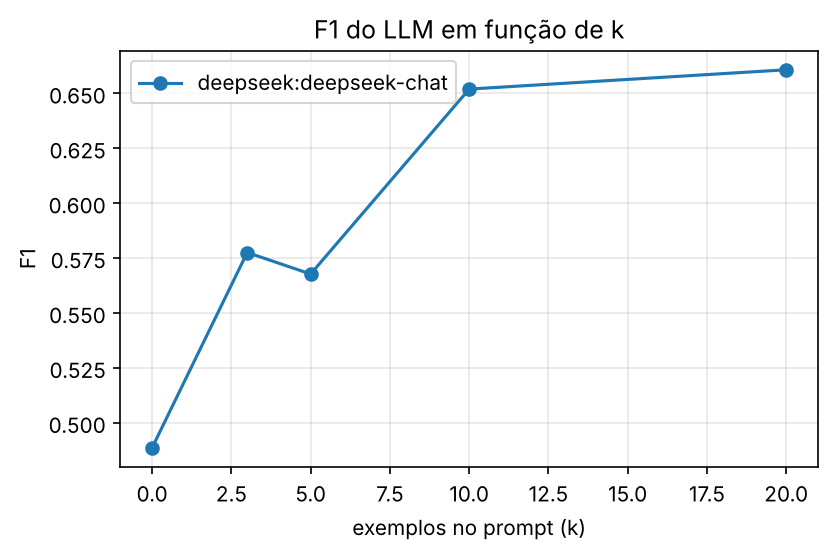
\includegraphics[width=.6\textwidth]{llm_f1_vs_k.png}
\caption{F1 do LLM na amostra fixa em função do número de exemplos $k$.}
\label{fig:fk}
\end{figure}

Quanto ao tempo, cada consulta levou em média 0,97~s, ou cerca de 96~s por 100 amostras, valor praticamente constante entre as configurações, já que é dominado pela ida e volta à API. Os tokens de entrada, em contrapartida, crescem de 272 para 1.560 por consulta, enquanto a saída fica fixa em 16, totalizando 764.800 tokens de entrada e 16.000 de saída. Assim, com os preços do \texttt{deepseek-v4-flash} consultados em 24/11/2026 (US\$~0,15 por milhão de tokens de entrada e US\$~0,60 de saída, fora do pico), o custo vai de US\$~0,005 a US\$~0,024 por 100 amostras e soma cerca de US\$~0,12, ou US\$~0,25 no pico. Note-se, ainda, que passar de 10 para 20 exemplos custa 70\% mais tokens sem ganho de F1.

% ---------------------------------------------------------------------------
\section{Comparação crítica}\label{sec:comparacao}

Colocando as duas etapas lado a lado na mesma amostra (Tabela~\ref{tab:comparacao} e Figura~\ref{fig:f1}), fica claro que mesmo a melhor configuração do LLM (F1 0,66) fica abaixo do pior modelo clássico (0,82) e mais de 0,2 abaixo da MLP e do XGBoost (0,88). Essa diferença, além disso, não é fruto do acaso: por \textit{bootstrap}, o intervalo de confiança de 95\% da diferença entre a MLP e o LLM com $k=20$ vai de 0,11 a 0,33. A AUC-ROC, por sua vez, segue o mesmo padrão, indo de 0,96 a 0,98 nos clássicos e não passando de 0,85 no LLM.

\begin{table}[ht]
\centering
\caption{Clássicos e LLM na amostra fixa (200 casos). Tempo dos clássicos só de inferência.}
\label{tab:comparacao}
\small
\begin{tabular}{llcccccc}
\toprule
Etapa & Modelo / configuração & Acur. & Prec. & Rev. & F1 & AUC & s/100 \\
\midrule
I  & MLP                      & 0,945 & 0,976 & 0,800 & 0,879 & 0,979 & 0,002 \\
I  & XGBoost                  & 0,945 & 0,976 & 0,800 & 0,879 & 0,973 & 0,003 \\
I  & SVM                      & 0,940 & 0,975 & 0,780 & 0,867 & 0,964 & 0,050 \\
I  & Random Forest            & 0,920 & 0,947 & 0,720 & 0,818 & 0,979 & 0,039 \\
\midrule
II & DeepSeek, $k=20$         & 0,810 & 0,597 & 0,740 & 0,661 & 0,843 & 96,6 \\
II & DeepSeek, $k=10$         & 0,765 & 0,518 & 0,880 & 0,652 & 0,850 & 95,0 \\
II & DeepSeek, \textit{zero-shot} & 0,550 & 0,341 & 0,860 & 0,489 & 0,721 & 97,7 \\
\bottomrule
\end{tabular}
\end{table}

\begin{figure}[ht]
\centering
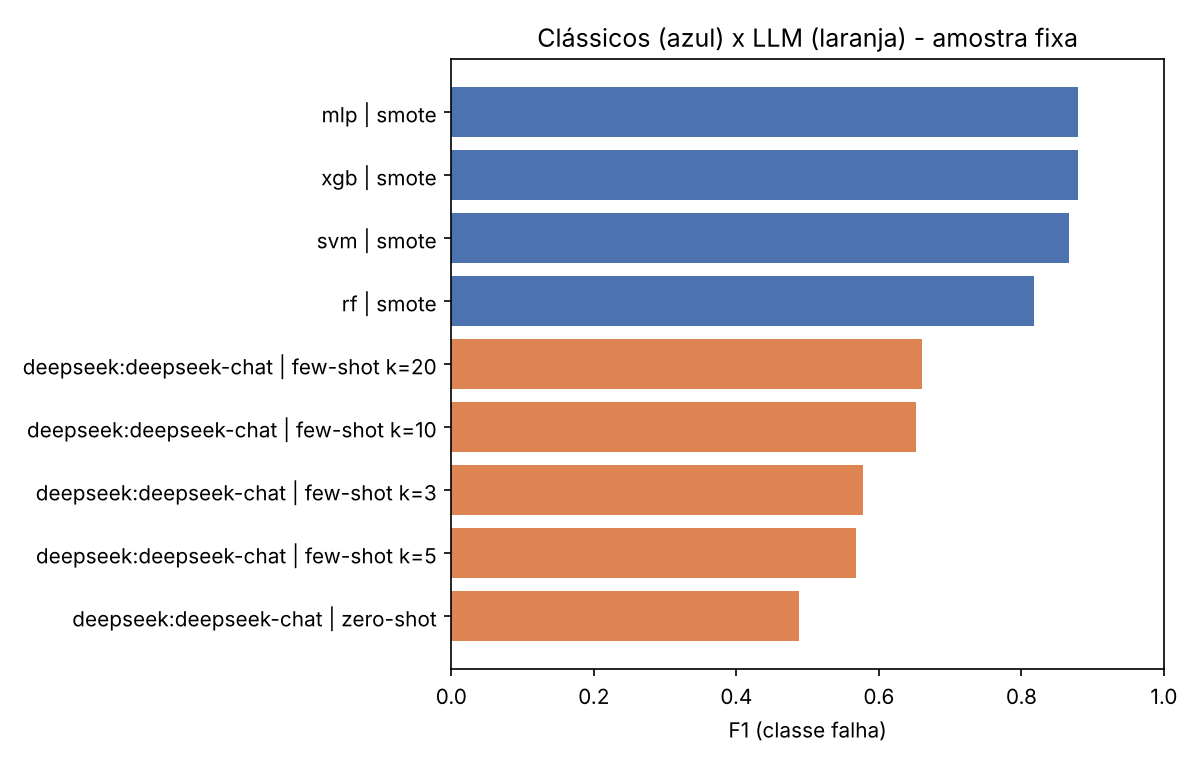
\includegraphics[width=.72\textwidth]{comparison_f1.png}
\caption{F1 da classe falha na amostra fixa: clássicos (azul) e LLM (laranja).}
\label{fig:f1}
\end{figure}

As matrizes da Figura~\ref{fig:cm} ajudam a entender onde cada abordagem erra. Enquanto a MLP emite apenas 1 alarme falso e perde 10 falhas, o LLM com $k=20$ emite 25 e, ainda assim, perde 13. Analisando as respostas, nota-se que os falsos positivos do LLM têm desgaste muito maior que os verdadeiros negativos (153 contra 47 min no \textit{zero-shot}); em outras palavras, o modelo aplica uma regra de senso comum, segundo a qual ferramenta gasta e torque alto indicam falha, que dispara em praticamente qualquer máquina desgastada. As regras reais da base, por outro lado, dependem de grandezas derivadas que o LLM teria de calcular sozinho. Curiosamente, há certa complementaridade, já que o LLM em \textit{zero-shot} detecta 9 das 10 falhas que a MLP deixa passar.

\begin{figure}[ht]
\centering
\begin{minipage}{.31\textwidth}\centering
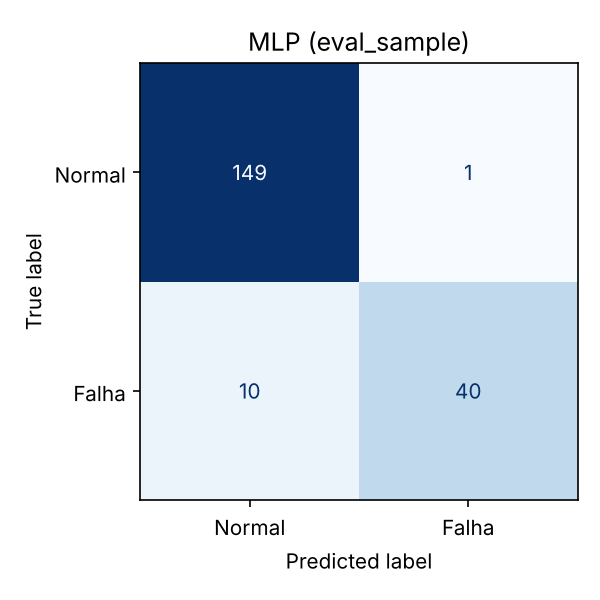
\includegraphics[width=\linewidth]{cm_mlp_eval_sample.png}\\{\footnotesize (a) MLP}
\end{minipage}\hfill
\begin{minipage}{.31\textwidth}\centering
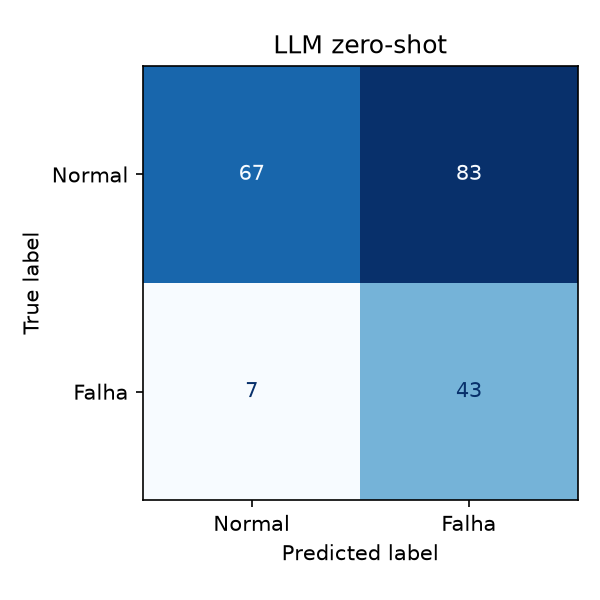
\includegraphics[width=\linewidth]{cm_llm_deepseek_deepseek-chat_k0.png}\\{\footnotesize (b) LLM \textit{zero-shot}}
\end{minipage}\hfill
\begin{minipage}{.31\textwidth}\centering
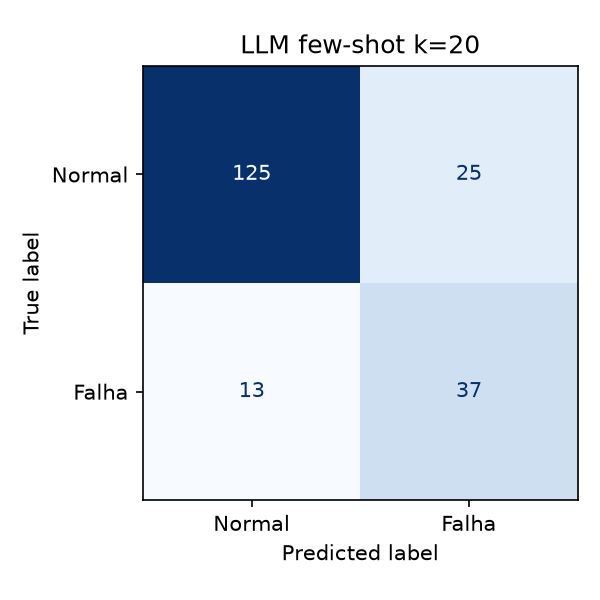
\includegraphics[width=\linewidth]{cm_llm_deepseek_deepseek-chat_k20.png}\\{\footnotesize (c) LLM, $k=20$}
\end{minipage}
\caption{Matrizes de confusão na amostra fixa (linhas: classe real; colunas: prevista).}
\label{fig:cm}
\end{figure}

Outro ponto que merece atenção é a qualidade das probabilidades do LLM, que são grosseiras, com apenas 9 a 13 valores distintos por configuração (no \textit{zero-shot}, por exemplo, 94 casos receberam 0,82), o que limita a AUC. Além disso, com $k=20$ o rótulo e a probabilidade se contradizem em 58 dos 200 casos, e só 58,5\% dos casos recebem a mesma resposta nas cinco configurações, o que revela grande sensibilidade ao \textit{prompt}. Por fim, quando se reestima a precisão para a taxa real de 3,4\% de falhas \cite{saito2015}, o LLM fica entre 0,05 (\textit{zero-shot}) e 0,14 ($k=20$), ou seja, seis de cada sete alarmes seriam falsos, contra 0,51 medidos para a MLP no teste completo.

Em resumo, cada abordagem tem vantagens e desvantagens próprias, que a Tabela~\ref{tab:pros} reúne.

\begin{table}[ht]
\centering
\caption{Pontos positivos e negativos de cada abordagem.}
\label{tab:pros}
\footnotesize
\begin{tabular}{>{\raggedright}p{2.6cm}>{\raggedright}p{5.3cm}>{\raggedright\arraybackslash}p{5.3cm}}
\toprule
 & Modelos clássicos & LLM via \textit{prompting} \\
\midrule
Desempenho & F1 0,82--0,88 na amostra; 0,76 no teste (XGB) & F1 0,49--0,66; muitos alarmes falsos \\
Dados & exigem milhares de exemplos rotulados & funcionam com 0 a 20 exemplos \\
Esforço & preparação, balanceamento e ajuste & descrição da tarefa em texto \\
Tempo e custo & milissegundos, sem custo por previsão & $\approx$1~s e US\$~0,00005--0,00024 por consulta \\
Privacidade & rodam localmente & dados enviados a API externa \\
Estabilidade & determinísticos & sensíveis ao \textit{prompt}; modelo pode mudar \\
\bottomrule
\end{tabular}
\end{table}

% ---------------------------------------------------------------------------
\section{Conclusões}\label{sec:conclusao}

Os resultados mostram que, quando há dados rotulados, os modelos clássicos vencem o LLM com folga nesta tarefa. Na mesma amostra, a MLP e o XGBoost alcançaram F1 de 0,88 contra 0,66 do DeepSeek, e o fizeram em uma fração do tempo e sem custo de inferência; no teste completo, além disso, o XGBoost obteve F1 de 0,76 com apenas 22 alarmes falsos em 2.000 ciclos. Por outro lado, o LLM se mostrou utilizável sem treino algum, detectando 86\% das falhas no \textit{zero-shot} e melhorando com exemplos até $k\approx10$. Portanto, sua melhor aplicação, neste cenário, é a de triagem inicial quando ainda não existem dados rotulados, e não a de substituto dos modelos treinados.

Esses resultados, contudo, devem ser lidos à luz de algumas limitações. Em primeiro lugar, a amostra tem apenas 50 falhas, de modo que o intervalo de confiança do F1 tem largura próxima de 0,2 e as diferenças entre as configurações com $k \geq 3$ não são significativas. Em segundo lugar, foram usados um único LLM, um único \textit{prompt}, um único sorteio de exemplos e uma única execução. Além disso, a base é sintética, regida por limiares simples e possivelmente vista no treino do LLM, e só os clássicos tiveram o limiar de decisão ajustado para o F1. Como próximos passos, propõe-se, portanto, incluir as grandezas derivadas no \textit{prompt}, escolher exemplos que cubram todos os modos de falha, repetir o experimento com várias sementes e ajustar o limiar sobre a probabilidade no treino; mais adiante, valeria ainda testar outros LLMs, recuperar exemplos semelhantes ao caso consultado (RAG) e combinar o LLM com os modelos clássicos.

% ---------------------------------------------------------------------------
\begin{thebibliography}{99}
\footnotesize
\setlength{\itemsep}{0pt}

\bibitem[Breiman 2001]{breiman2001}
Breiman, L. (2001). Random forests. \textit{Machine Learning}, 45(1):5--32.

\bibitem[Brown et al. 2020]{brown2020}
Brown, T. et al. (2020). Language models are few-shot learners. In \textit{NeurIPS 2020}, p. 1877--1901.

\bibitem[Chawla et al. 2002]{chawla2002}
Chawla, N. V., Bowyer, K. W., Hall, L. O. e Kegelmeyer, W. P. (2002). SMOTE: synthetic minority over-sampling technique. \textit{JAIR}, 16:321--357.

\bibitem[Chen e Guestrin 2016]{chen2016}
Chen, T. e Guestrin, C. (2016). XGBoost: a scalable tree boosting system. In \textit{KDD 2016}, p. 785--794.

\bibitem[Cortes e Vapnik 1995]{cortes1995}
Cortes, C. e Vapnik, V. (1995). Support-vector networks. \textit{Machine Learning}, 20(3):273--297.

\bibitem[DeepSeek 2026]{deepseek2026}
DeepSeek (2026). DeepSeek API Docs: models \& pricing e change log. \url{https://api-docs.deepseek.com/quick_start/pricing}. Acesso em: 24 nov. 2026.

\bibitem[Haykin 2009]{haykin2009}
Haykin, S. (2009). \textit{Neural Networks and Learning Machines}. Pearson, 3. ed.

\bibitem[Hegselmann et al. 2023]{hegselmann2023}
Hegselmann, S. et al. (2023). TabLLM: few-shot classification of tabular data with large language models. In \textit{AISTATS 2023}, p. 5549--5581.

\bibitem[Lemaître et al. 2017]{lemaitre2017}
Lemaître, G., Nogueira, F. e Aridas, C. K. (2017). Imbalanced-learn: a Python toolbox to tackle the curse of imbalanced datasets in machine learning. \textit{JMLR}, 18(17):1--5.

\bibitem[Matzka 2020a]{matzka2020}
Matzka, S. (2020a). Explainable artificial intelligence for predictive maintenance applications. In \textit{AI4I 2020}, p. 69--74. IEEE.

\bibitem[Matzka 2020b]{matzka2020uci}
Matzka, S. (2020b). AI4I 2020 Predictive Maintenance Dataset. UCI Machine Learning Repository. \url{https://doi.org/10.24432/C5HS5C}.

\bibitem[Pedregosa et al. 2011]{pedregosa2011}
Pedregosa, F. et al. (2011). Scikit-learn: machine learning in Python. \textit{JMLR}, 12:2825--2830.

\bibitem[Saito e Rehmsmeier 2015]{saito2015}
Saito, T. e Rehmsmeier, M. (2015). The precision-recall plot is more informative than the ROC plot when evaluating binary classifiers on imbalanced datasets. \textit{PLOS ONE}, 10(3):e0118432.

\end{thebibliography}

\end{document}
